\chapter{
شمارنده BCD
}

در این قسمت باید از قطعه از شمارنده‌ی 
BCD
داده شده استفاده کنیم.

کافی است خروجی که نشان دهنده‌ی تمام شدن یک سیکل در شمارنده‌ی اول است را به کلاک شمارنده‌ی دوم وصل کنیم.
با این کار با به ۱۰ رسیدن شمارنده‌ی اول
(که یعنی همان ۰ شدنش)
شمارنده‌ی بعدی یکی زیاد می‌شود که مطابق انتظار ما است.

در انتها باید هنگامی که شمارنده‌ها به
64
می‌رسند آن‌ها را ریست کنیم.
برای این کار کافی
64
شدن بیت‌ها را چک کنیم.
اما می‌دانیم مقدار این اعداد از
4 و 
6
بیشتر نمی‌شود.
پس کار ما خیلی راحت‌تر می‌شود و مطابق نتیجه‌ی نهایی در شکل
\eqref{fig:circuit4}
می‌توانیم تنها با چک کردن
3 بیت
این کار را انجام دهیم.


\begin{figure}
    \centering
    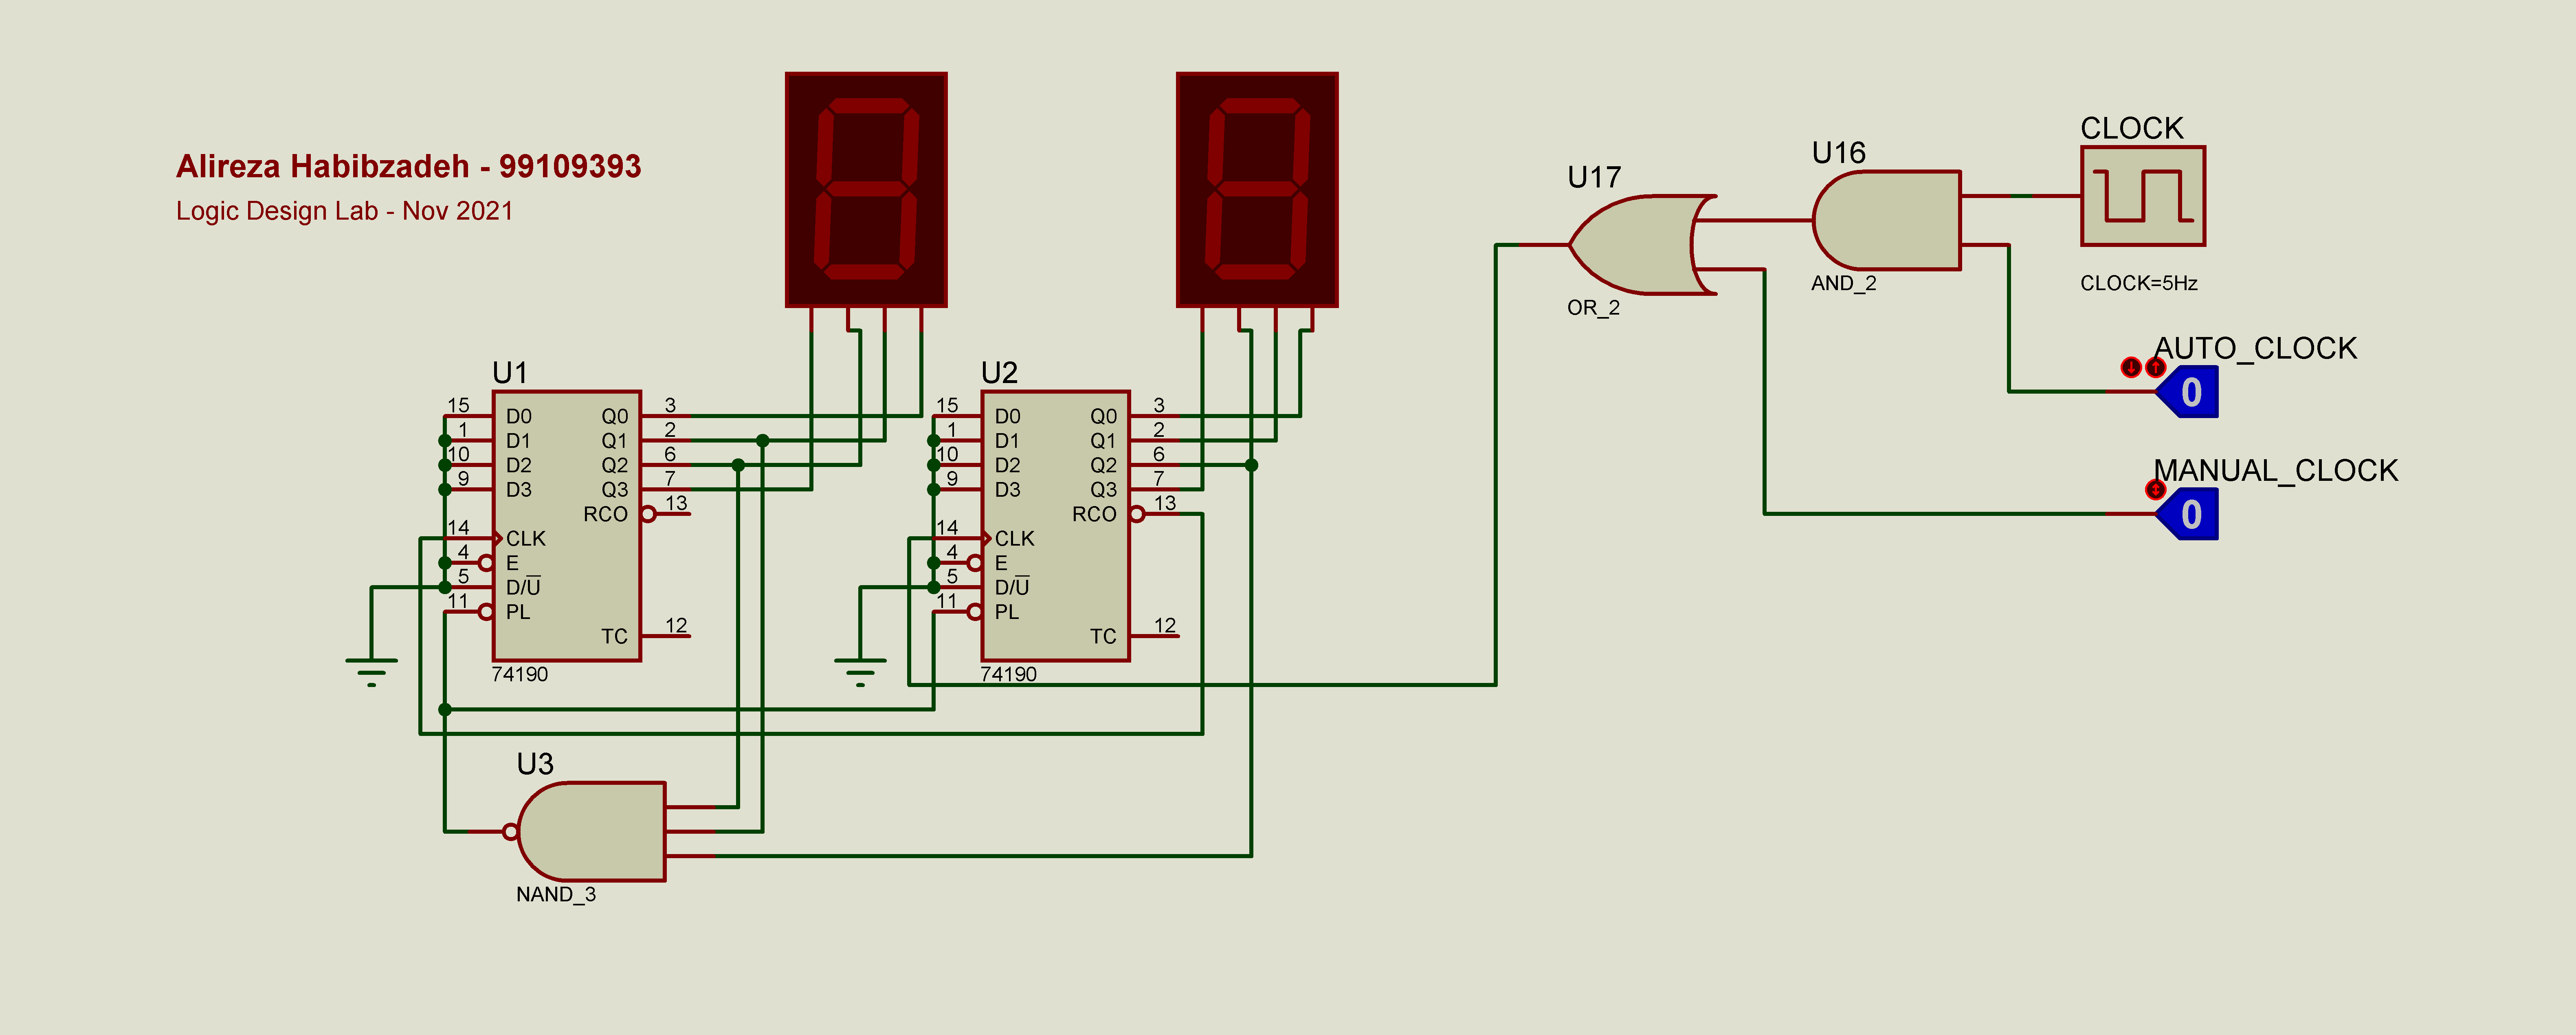
\includegraphics[width=\textwidth]{part3/3.png}
    \caption{
    شمارنده BCD
    تا ۶۳
    }
    \label{fig:circuit4}
\end{figure}